%\documentclass{tikzposter}
\documentclass[25pt, a0paper,
%landscape,
margin=0mm, innermargin=15mm, blockverticalspace=5mm, colspace=15mm, subcolspace=6mm]{tikzposter}
\usepackage{trace}
\usepackage{amsmath}
\usepackage{mathtools}
\usepackage[no-math]{fontspec}
\usepackage[vargreek-shape=unicode]{unicode-math}
%\RequirePackage{lualatex-math}
\newfontfeature{Microtype}{protrusion=default;expansion=default;}
\tikzposterlatexaffectionproofoff

% Maths
\setmathfont{XITS Math}
%\setmathfont{Asana Math}
%\setmathfont{Cambria Math}
%\setmathfont{Neo Euler}
%\setmathfont[range={"02660-"0266F}]{Asana Math}
%\setmathfont[range={"02420-"0242F}]{Asana Math}

% Futura
% \setmainfont[Renderer=Basic,Microtype,Ligatures=TeX]{Futura Std}
% \setsansfont[Scale=MatchLowercase
% %,Mapping=tex-text
% ,Ligatures=TeX
% ,BoldFont=*Bold%
% ,BoldItalicFont=*BoldOblique%
% ,ItalicFont=*BookOblique%
%  ]{Futura Std}
% \setmathfont[range=\mathit/{latin,Latin}, Scale=MatchUppercase]{Futura Std Book Oblique}

% Optima
\setmainfont[Renderer=Basic,Microtype,Ligatures=TeX,
BoldFont=*Bold%
,BoldItalicFont=*BoldItalic%
,ItalicFont=*Italic%
]{OptimaLT Std}
% \setsansfont[Scale=MatchLowercase
% %,Mapping=tex-text
% ,Ligatures=TeX
% ,BoldFont=OptimaLTStdBlack%
% ,BoldItalicFont=OptimaLTStdBlackItalic%
% ,ItalicFont=*Italic%
%  ]{OptimaLT Std DemiBold}

\setmathfont[range=\mathit/{latin,Latin},
Scale=MatchUppercase]{OptimaLT Std DemiBold Italic}

% tt
\setmonofont[Scale=MatchLowercase]{Consolas}


%\setmainfont[Renderer=Basic,Microtype,Ligatures=TeX]{Futura Std}
%\setmainfont[Microtype,Ligatures=TeX]{Constantia}
%\setsansfont[Ligatures=TeX,Scale=MatchLowercase]{Calibri}


%\setmathfont[Numbers=Lining, Scale=MatchUppercase]{Futura Std}


%\def\mathvisiblespace{\mathchar"02FD}

\usepackage{graphicx}
\usepackage{hyperref}
\newcommand{\email}[1]{\href{mailto:#1}{\textsf{#1}}}
%\usepackage{url}
\title{\parbox{\linewidth}{\begin{center}\textbf{A Heuristic Method for Large-Scale Cognitive-Diagnostic}\\ \textbf{Computerized Adaptive Testing}\end{center}}}
%\titlegraphic{\includegraphics[width=0.7\textwidth]{Logo_Supelec}}
\author{\centering
  \begin{tabular}{ccccc}
    \textbf{Jill-Jênn Vie} & \textbf{Fabrice Popineau} & \textbf{Françoise Tort} & \textbf{Benjamin Marteau} & \textbf{Nathalie Denos} \\
    RIKEN Center for Advanced & Laboratoire de recherche & ENS Paris-Saclay & French Ministry of Education & Université Grenoble-Alpes\\
Intelligence Project (AIP) & en informatique (LRI) & Cachan, France & Paris, France & Grenoble, France \\
Tokyo, Japan & Orsay, France &  \texttt{francoise.tort} & \texttt{benjamin.marteau} & \texttt{nathalie.denos} \\
\texttt{vie@jill-jenn.net} & \texttt{fabrice.popineau@lri.fr} & \texttt{@stef.ens-cachan.fr} & \texttt{@education.gouv.fr} & \texttt{@univ-grenoble-alpes.fr}
  \end{tabular}
    }
%\institute{\raggedleft SUPELEC Systems Sciences (E3S), Computer Science Department, Gif-sur-Yvette, France \\[8mm]
%  \hfill \email{\{fabrice.popineau,georges.dubus,yolaine.bourda\}@supelec.fr}
%}

%\usetheme{Basic}
\usetheme{Simple}
%\usetheme{Wave}
%\usetitlestyle{VerticalShading}
%\usebackgroundstyle{VerticalGradation}
%\usebackgroundstyle{Rays}
\usecolorpalette{BrownBlueOrange}
\makeatletter
\renewcommand\TP@maketitle{%
  % \begin{minipage}{0.06\linewidth}
  %   \centering
  %   
\includegraphics[width=0.8\textwidth]{figures/logo-cs.png}\\[1em]
  %   
\includegraphics[width=0.8\textwidth]{figures/logo-men.pdf}
  % \end{minipage}
   \begin{minipage}{0.98\linewidth}
        \centering
        \color{titlefgcolor}
        {\bfseries \Huge \sc \@title \par}
        \vspace*{1em}
        {\Large
          \@author \par}
    \end{minipage}%
    % \hfill
    % \begin{minipage}{0.06\linewidth}
    %   \centering
    % 
\includegraphics[width=0.8\textwidth]{figures/logo-ensps.jpg}\\[1em]
    % 
\includegraphics[width=0.8\textwidth]{figures/logo-lri.pdf}
    % \end{minipage}
}
\makeatother

\usepackage{theorem}
\theoremstyle{myplain}
\newtheorem{transformation}{Transformation}
% \newtheorem{theorem}{Theorem}
%\theoremstyle{definition}
% \newtheorem{definition}{Definition}
\newcommand{\concprio}{\rangle\kern-0.15em\rangle}

%\usepackage{tikz}
\usepackage{tikz-qtree}

%\setbeameroption{show notes}
\usetikzlibrary{arrows,arrows.meta,automata,shapes,intersections,mindmap,trees,shadows,fit,positioning,calc,matrix,decorations,chains,external,3d}
\makeatletter
\tikzoption{canvas is xy plane at z}[]{%
\def\tikz@plane@origin{\pgfpointxyz{0}{0}{#1}}%
\def\tikz@plane@x{\pgfpointxyz{1}{0}{#1}}%
\def\tikz@plane@y{\pgfpointxyz{0}{1}{#1}}%
\tikz@canvas@is@plane
}
\makeatother
\usepackage{listings}
\usepackage{enumitem}
\usepackage{booktabs}
\newcommand{\Gproc}{\textbf{proc }}
\newcommand{\GendProc}{\textbf{ endProc}}
\newcommand{\Gif}{\textbf{if }}
\newcommand{\Gthen}{\textbf{ then }}
\newcommand{\Gelse}{\textbf{ else }}
\newcommand{\Gwhile}{\textbf{while }}
\newcommand{\Gdo}{\textbf{ do }}
\newcommand{\mprefer}{\,\rangle\,}
\newcommand{\GendIf}{\textbf{ endIf }}
\newcommand{\GendWhile}{\textbf{ endWhile }}
\newcommand{\affp}{\textit{aff\/}_p}
\newcommand{\set}[1]{\{#1\}}

\newcommand{\Gleft}[1]{G_{#1}^{\textit{left}}}
\newcommand{\Gright}[1]{G_{#1}^{\textit{right}}}
\newcommand{\Gmiddle}[1]{G_{#1}}

\newcommand{\prefer}{\rangle}

\newcommand{\alert}[1]{{\color{red!70!black} #1}}

\newcommand{\bs}{\textbackslash}   % backslash
\newcommand{\cmd}[1]{{\bf \color{red}#1}}   % highlights command

\graphicspath{{./}{../images/}}

%\usenotestyle{Corner}
%\usenotestyle{VerticalShading}
\usenotestyle{Sticky}
\begin{document}
\maketitle[width=\linewidth,titletotopverticalspace=0pt]

% Here it starts

\definecolor{pixblue}{RGB}{53,81,250}
\colorlet{innerblocktitlebgcolor}{pixblue}

\begin{columns} % Blocks will be placed into columns
    
    \column{.55}
    \block[roundedcorners=40]{Context: Cognitive-Diagnostic Computerized Adaptive Testing}{
        \textbf{Input:} a dependency graph between \textbf{knowledge components} (KC)\\
        \textbf{Output:} an adaptive test (CAT tree) with feedback
        \begin{itemize}
            \item \textbf{Adaptive testing} $\Rightarrow$ personalized assessment
            \item \textbf{Formative testing} $\Rightarrow$ need of feedback (using the KCs)
            \item \textbf{Many knowledge components} $\Rightarrow$ standard methods do not apply
            \item \textbf{Cold-start} $\Rightarrow$ no user data available yet
        \end{itemize}

        \vspace{1cm}
        \innerblock[]{Item Response Theory}{
            Students $i \in I$ have \textbf{unknown} level $\theta_i$\\
            Questions $j \in J$ have difficulty $d_j$ (potentially calibrated on data)
            \[ \Pr(\textsf{correct}_{ij}) \triangleq \Pr(\textsf{student}_i \textnormal{ answers correctly } \textsf{question}_j) \triangleq \frac1{1 + e^{-(\theta_i - d_j)}} \]
            \hfill $\Rightarrow$ \textnormal{ \textbf{$\theta$ is easily estimated, but no feedback}}
        }
        \vspace{1cm}
        \innerblock[]{DINA \& Attribute Hierarchy Model}{
            Knowledge components $1, \ldots, K$\\
            Students $i \in I$ have \textbf{unknown} knowledge $\in \{0, 1\}^K$\\
            Questions $j \in J$ have requirements $\in \{0, 1\}^K$ (q-matrix), slip $s_j$ and guess $g_j$ parameters
            \[ \Pr(\textsf{correct}_{ij}) \triangleq \left\{\begin{array}{cl}
1 - s_j & \textnormal{if } \textsf{student}_i \textnormal{ masters the requirements of } \textsf{question}_j\\
g_j & \textnormal{otherwise.}
\end{array}\right. \]
            \hfill $\Rightarrow$ \textnormal{ \textbf{can be used in cold-start, but not scalable when $K$ grows ($\geq$ 50)}}
        }
    }

    \block{Can we do better?}{
        \innerblock[]{Our Heuristic Method}{
            \raggedright
            Knowledge components $1, \ldots, K$ contain a \textbf{tag} and a \textbf{difficulty} level (ex. \texttt{@url4})\\
            \raggedleft KCs are linked in a \textbf{dependency graph}\\
            \raggedright Students $i \in I$ have unknown \textbf{level} $\theta_i$ and knowledge $\in \{0, 1\}^K$\\
            Questions $j \in J$ have a unique main requirement $\in \{1, \ldots, K\}$\\
            \raggedleft $\Pr(\textsf{correct}_{ij})$ is same as in Item Response Theory
            \[ score(j) = \Pr(\textsf{correct}_{ij}) \cdot N_{\textsf{acquired nodes if correct}} + \Pr(\textsf{incorrect}_{ij}) \cdot N_{\textsf{non-acquired nodes if incorrect}} \]
        }
        \begin{itemize}
            \item \textbf{Rough estimate of the number of nodes marked} in the dependency graph at each step
            \item \textbf{Greedy selection} to build the tree
            \item Later in the test, we can \textbf{switch to a more precise diagnostic model}
            \item \textbf{Add edges to dependency graph} based on usage (Deep Knowledge Tracing, NIPS 2015)
        \end{itemize}
    }

    % \block{Example}{
    %     \centerline{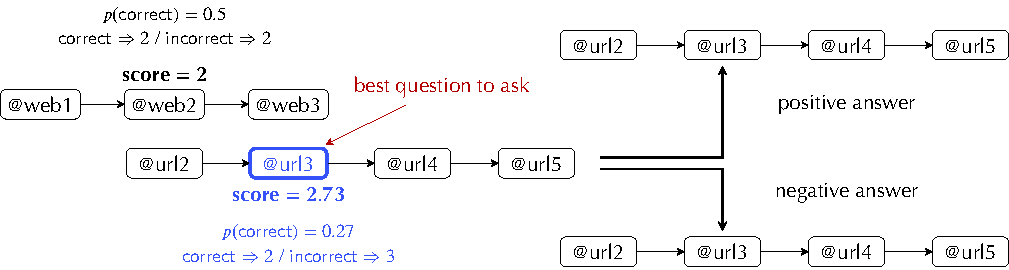
\includegraphics[width=0.8\linewidth]{figures/example.pdf}}
    % }

    % \block{Impact}{
    %     \begin{itemize}
    %         \item \textbf{800 exercises} based on evidence-centered design
    %         \item \textbf{3.5 million} high school students (grade 8 to 12)
    %         \item \textbf{1.25 million} higher-education students
    %         \item The platform is on GitHub (license AGPLv3)
    %     \end{itemize}
    % }

    \column{.45}
    \block{Output: Computerized Adaptive Testing (CAT)}{
        The next question is chosen based on the answer history.

        \vspace{1cm}
        \centerline{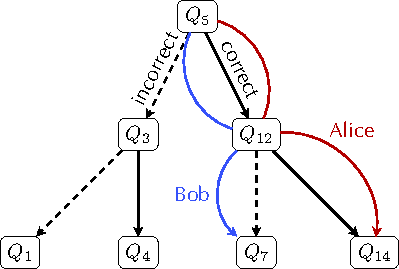
\includegraphics[width=0.6\linewidth]{figures/adaptive.pdf}}
    }

    \block{Input: Dependency Graph over DIGCOMP 2.0}{
      % 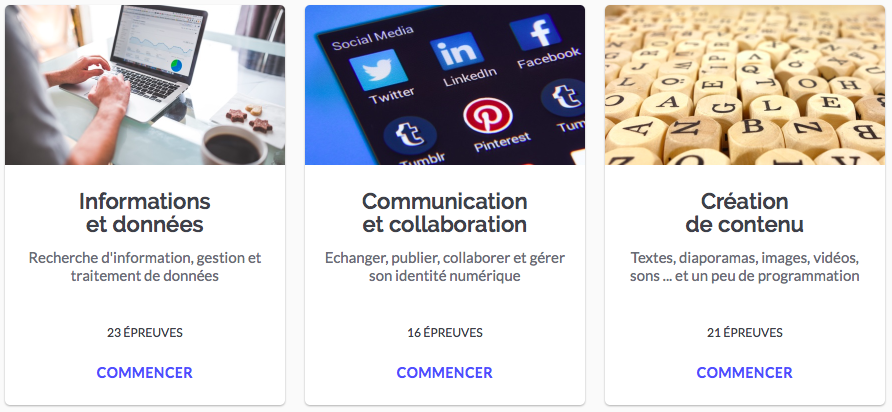
\includegraphics[width=\linewidth]{figures/domains.png}
      % \begin{minipage}{0.4\textwidth}
      %   5 domains of the DIGCOMP referential for numerical competencies \\
      %   \begin{itemize}
      %   \item Information \& Data Literacy
      %   \item Communication \& Collaboration
      %   \item Digital Content Creation
      %   \item Safety
      %   \item Problem Solving
      %   \end{itemize}
      % \end{minipage}
      % \hfill
      % \begin{minipage}[c]{0.55\textwidth}
      \centerline{
      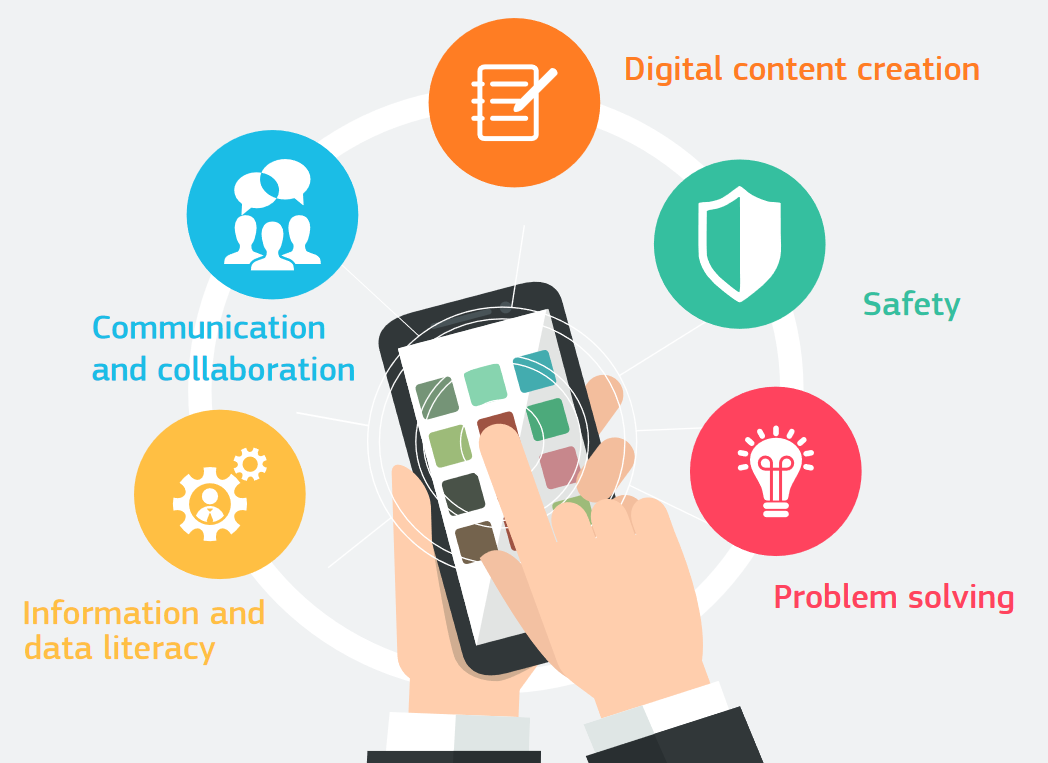
\includegraphics[width=0.25\textwidth]{figures/digcomp-2.png}
      }
      % \end{minipage}
      Tags are related to these domains.\\
        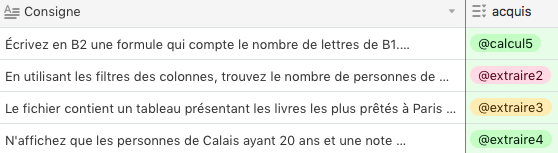
\includegraphics[width=\linewidth]{figures/tags.png}
        % \begin{itemize}
        %     \item Each validation triggers the validation of parents.
        %     \item Each non-validation triggers the non-validation of children.
        % \end{itemize}
        % 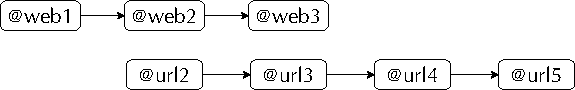
\includegraphics[width=\linewidth]{figures/example2.pdf}
        % 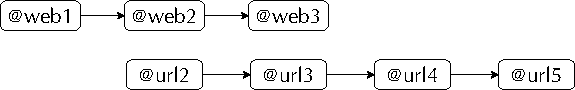
\includegraphics[width=\linewidth]{figures/example2.pdf}
    }

    % \block{Output: Example of CAT tree}{
    %     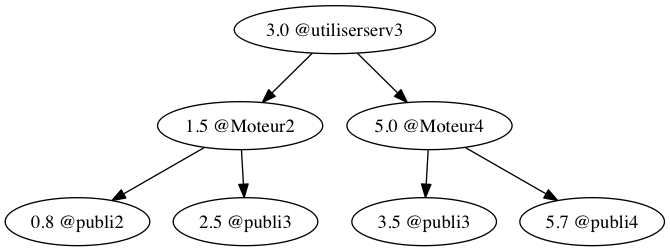
\includegraphics[width=\linewidth]{figures/cat.png}
    % }

\end{columns}
\block{Example}{
  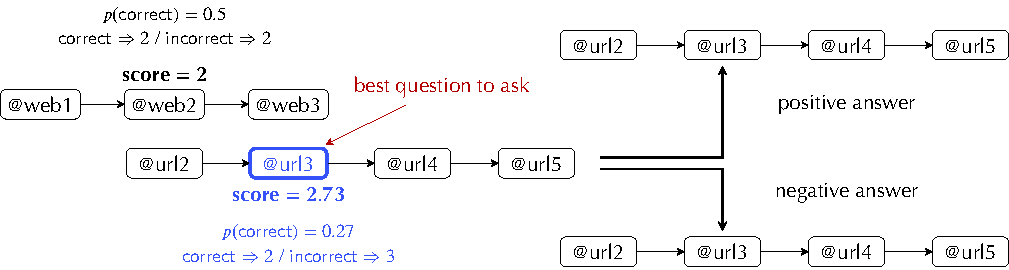
\includegraphics[width=0.62\linewidth]{figures/example.pdf}
  \hfill
  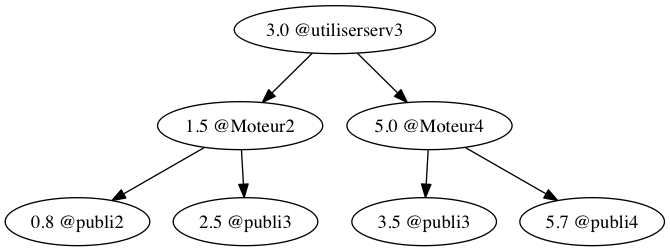
\includegraphics[width=0.33\linewidth]{figures/cat.png}
}

\block{Application: Certifying the Digital Competencies of French citizens}{
    \begin{minipage}[b]{0.4\linewidth}
        \begin{itemize}
            \item \textbf{800 skeletons of exercises} based on evidence-centered design
            \item \textbf{800 knowledge components}
            \item \textbf{3.5 million} high school students (grade 8 to 12)
            \item \textbf{1.25 million} higher-education students
            \item The platform is on GitHub (license AGPLv3)
        \end{itemize}
    \end{minipage}
    \begin{minipage}[b]{0.4\linewidth}
      \raisebox{-2cm}{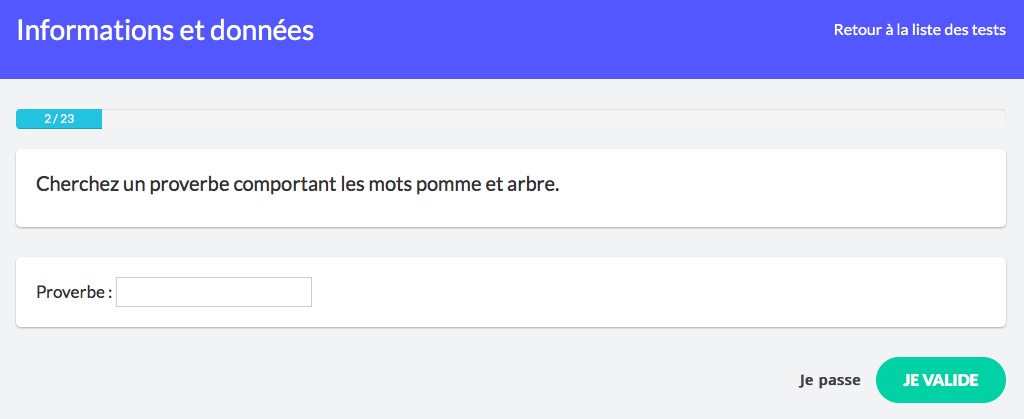
\includegraphics[width=\linewidth]{figures/pix.png}}
    \end{minipage}
    \hfill
    \begin{minipage}[b]{0.08\linewidth}
      \centering
    
\includegraphics[width=0.8\textwidth]{figures/logo-ensps.jpg}\\[1em]
    
\includegraphics[width=0.8\textwidth]{figures/logo-lri.pdf}
    \end{minipage}
    \hfill
    \begin{minipage}[b]{0.08\linewidth}
      \centering
      
\includegraphics[width=0.8\textwidth]{figures/logo-cs.png}\\[1em]
      
\includegraphics[width=0.8\textwidth]{figures/logo-men.pdf}
    \end{minipage}

}

\end{document}

\endinput

%%% Local Variables:
%%% mode: latex
%%% TeX-master: t
%%% End:
